\documentclass[12pt]{article}

\usepackage{color}
\usepackage[portuguese]{babel}
\usepackage[utf8]{inputenc}
\usepackage{indentfirst}
\usepackage{graphicx}
\usepackage{verbatim}
\usepackage{listings}
\usepackage{url}
\usepackage{stringenc}
\usepackage{pdfescape}
\usepackage{subfig}
\usepackage{float}
\usepackage{eurosym}
\begin{document}

\setlength{\textwidth}{16cm}
\setlength{\textheight}{22cm}
\title{\huge\textbf{\textit{Enterprise Distributed Application}}\linebreak
\Large\textbf{\\Trabalho \#2}\linebreak\linebreak\linebreak

\includegraphics[width=8cm]{feup.pdf}\linebreak \linebreak
\large{Mestrado Integrado em Engenharia Informática e Computação} \linebreak
\large{Tecnologias de Distribuição e Integração \\ EIC0077-2S}\linebreak
}
\author{
João Carlos Teixeira de Sá - 201107925 (ei11142@fe.up.pt)\\
João Pedro Matos Teixeira Dias - 201106781 (ei11137@fe.up.pt)\\
\\
\\ Faculdade de Engenharia da Universidade do Porto \\ Rua Roberto Frias, s\/n, 4200-465 Porto, Portugal
 \vspace{1cm}}
%\date{Junho de 2007}
\maketitle
\thispagestyle{empty}

%************************************************************************************************
%************************************************************************************************

\newpage

\tableofcontents

%************************************************************************************************
%************************************************************************************************

%*************************************************************************************************
%************************************************************************************************

\newpage

\section{Introdução}

O presente documento apresenta o desenvolvimento do projeto \textit{Enterprise Distributed Application} para a unidade curricular de Tecnologias de Distribuição e Integração. 

O projeto tem como objetivo o desenvolvimento de um sistema, \textit{Enterprise Distributed Application}, capaz de gerir compras e vendas de livros de uma editora (\textit{diginotes}). 

O sistema é composto por um servidor presente numa loja que persiste a informação relativa aos livros existentes para venda tais como o título, preço e o stock disponível tanto na loja como em armazém. Este servidor encontra-se ligado à \textit{internet} e está sempre disponível.

As compras de um livro por parte de um consumidor podem ser feitas diretamente na loja ou através de uma aplicação \textit{web}. Caso exista stock do livro pretendido o mesmo é imediatamente entregue ao consumidor no caso da compra ser feita na loja ou enviado pelo correio caso seja efetuado o pedido através da aplicação \textit{web}; no caso de não existir stock a loja deve enviar uma mensagem para o armazém a pedir o envio do livro em questão numa quantidade 10 vezes superior ao pretendido pelo cliente.


\section{Tecnologias}

O projeto foi desenvolvido usando a \textit{framework Windows Communication Foundation} para o desenvolvimento da API disponibilizada da loja bem como a tecnologia \textit{Microsoft Message Queuing} para o envio e receção das mensagens de pedido de stock de livros ao armazém utilizando em ambos os casos a linguagem de programação C\#. Além disso foram também utilizadas as linguagens de programação PHP, HTML  e Javascript para o desenvolvimento da aplicação \textit{web}. 

Adicionalmente foi utilizado para persistência de dados a tecnologia de base de dados \textit{MongoDB} e para o desenvolvimento da interfaces de utilizador da loja e do armazém a tecnologia \textit{Windows Presentation Foundation} usando a linguagem \textit{XAML}.

Por último, para gestão de dependências do projeto foi usado o \textit{NuGet} e para gestão de versões foi utilizada a ferramenta \textit{Git} usando a plataforma \textit{GitHub}.


\section{Arquitetura}

\begin{figure}[h!]
    \centering
    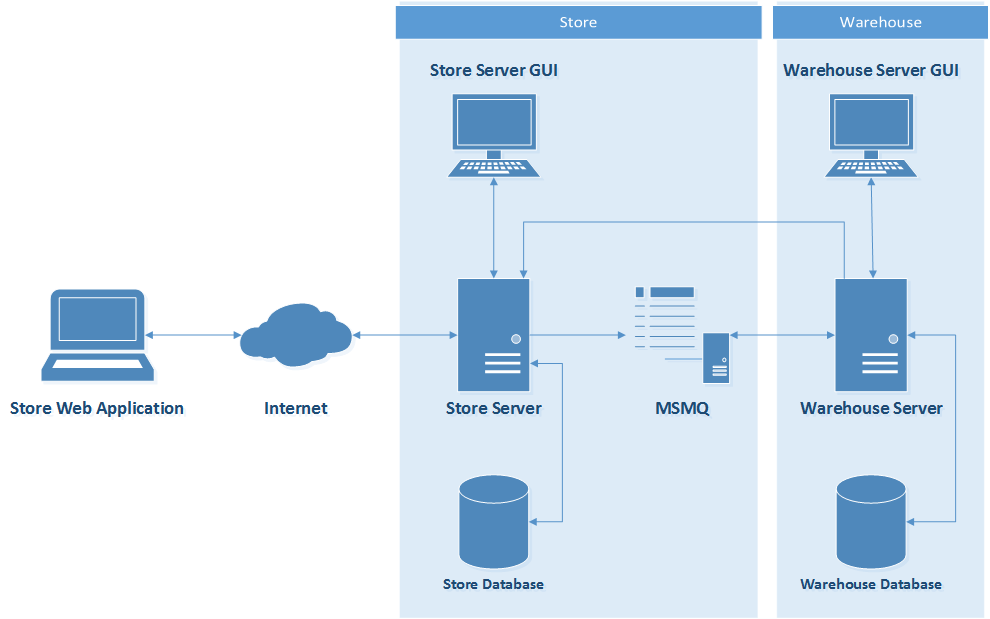
\includegraphics[width=0.8\textwidth]{arch.png}
    \caption{Arquitetura do Sistema.}
    \label{fig:arch}
\end{figure}

O sistema apresenta a estrutura típica de um projeto baseado em \textit{Windows Communication Foundation}, como representado na fig. \ref{fig:arch}, contando assim com um servidor da loja que disponibiliza um API que pode ser acedida por aplicações clientes, neste caso uma aplicação com interface gráfica presente na loja e uma aplicação disponível na \textit{web}. Além disso existe também um servidor no armazém que recebe e trata mensagens de pedidos de stock provenientes da loja. Acrescenta-se ainda uma persistência de dados tanto na loja como no armazém existindo uma base de dados MongoDD associada a cada um dos servidores.

\begin{figure}[h!]
    \centering
    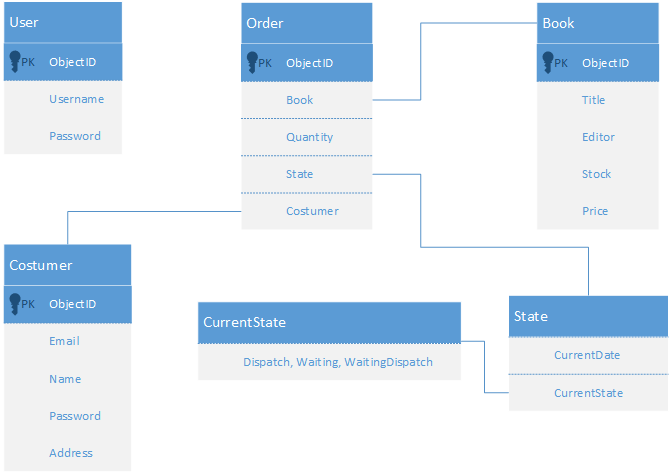
\includegraphics[width=0.5\textwidth]{DBStore.png}
    \caption{Esquema da base de dados da loja.}
    \label{fig:arch}
\end{figure}

\ref{fig:DBStore}

\begin{figure}[h!]
    \centering
    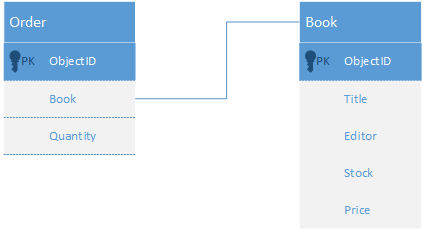
\includegraphics[width=0.5\textwidth]{DBWarehouse.png}
    \caption{Esquema da base de dados do armazém.}
    \label{fig:arch}
\end{figure}

\ref{fig:DBWarehouse}

\newpage

Apresenta-se também com uma divisão modular apresentando:
\begin{itemize}
\item Módulo comum
\begin{itemize}
\item Definição das estruturas de dados partilhadas entre cliente e servidor.
\end{itemize}
\item Módulo cliente
\begin{itemize}
\item Aplicação com interface gráfica para a loja.
\item Aplicação \textit{web}.
\end{itemize}
\item Módulo servidor (da loja)
\begin{itemize}
\item Aplicação com lógica do sistema, transações e persistência de dados.
\item Disponibilização de uma API para consulta pelas aplicações cliente.
\end{itemize}
\item Módulo servidor (do armazém)
\begin{itemize}
\item Aplicação  para receção e tratamento de mensagens de pedidos de stock por parte da loja.
\item Aplicação com interface gráfica para os funcionários do armazém.
\end{itemize}
\end{itemize}

O sistema ainda utiliza objetos para representação das transações (\textit{order}), dos livros (\textit{book}) e para a informação dos clientes (\textit{costumer}) bem como dos utilizadores das aplicações com interface gráfica da loja e do armazém (\textit{user}).


\section{Front-end}

\subsection{Interface gráfica da aplicação da loja}

\begin{figure}[H]
    \centering
    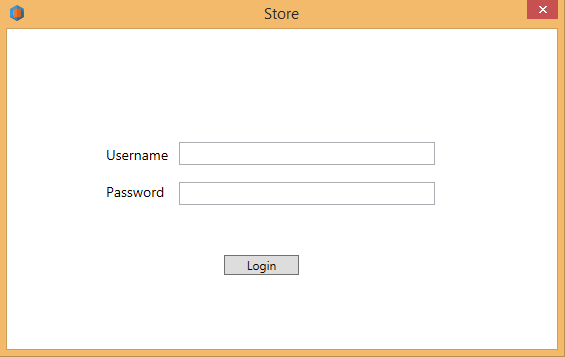
\includegraphics[width=0.8\textwidth]{Store_GUI_Login.png}
    \caption{Interface gráfica da aplicação da loja - \textit{Login.}}
    \label{fig:c1}
\end{figure}

Ao nível da interface gráfica desenvolvida para a aplicação presente na loja é disponibilizada numa primeira fase um ecrã de \textit{login}, fig. \ref{fig:c1}, onde o funcionário da loja pode entrar no sistema.

Após o funcionário fazer \textit{login} no sistema são disponibilizadas as opções de criar uma venda e de verificar quais as encomendas efetuadas através da aplicação \textit{web} podendo estas serem marcadas como enviadas após o envio para o cliente, fig. \ref{fig:c2} e \ref{fig:c3}.

Por último, no momento em que é criada uma venda o sistema questiona o funcionário se pretende imprimir uma fatura, fig. \ref{fig:c4}, sendo esta exportada para um ficheiro pdf em caso afirmativo.

\begin{figure}[H]
    \centering
    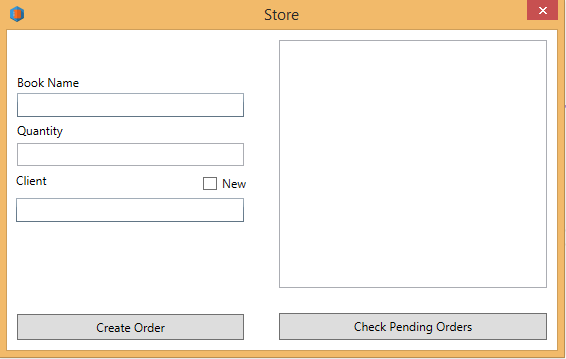
\includegraphics[width=0.8\textwidth]{Store_GUI_Main.png}
    \caption{Interface gráfica da aplicação da loja - Ecrã principal.}
    \label{fig:c2}
\end{figure}
\begin{figure}[H]
    \centering
    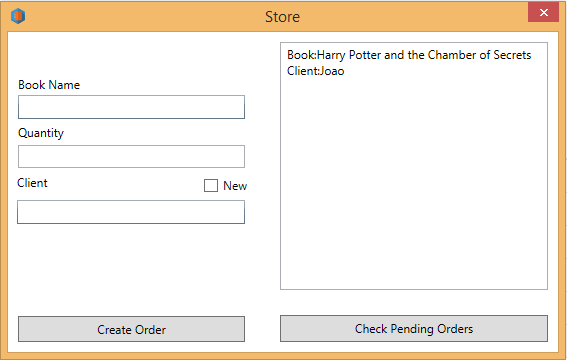
\includegraphics[width=0.8\textwidth]{Store_GUI_Order_Pending.png}
    \caption{Interface gráfica da aplicação da loja - Ecrã principal com encomenda pendente.}
    \label{fig:c3}
\end{figure}
\begin{figure}[H]
    \centering
    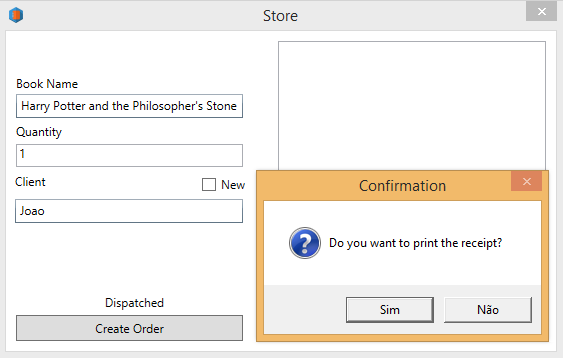
\includegraphics[width=0.8\textwidth]{Store_GUI_Receipt_Confirmation_Dialog.png}
    \caption{Interface gráfica da aplicação da loja - Confirmação de impressão de fatura de uma venda.}
    \label{fig:c4}
\end{figure}

\subsection{Interface gráfica da aplicação do armazém}

\begin{figure}[H]
    \centering
    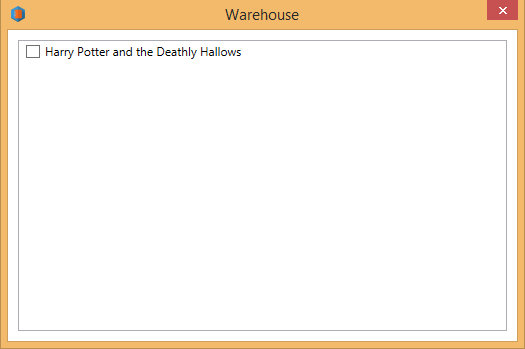
\includegraphics[width=0.8\textwidth]{Warehouse_GUI_Main.png}
    \caption{Interface gráfica da aplicação do armazém - Ecrã principal.}
    \label{fig:c5}
\end{figure}

Ao nível da interface gráfica desenvolvida para a aplicação presente no armazém esta contém apenas uma janela em que é disponibilizada uma lista de pedidos de livros por parte da loja devendo o funcionário do armazém colocar um visto num pedido quando os livros correspondentes a esse pedido forem enviados para a loja, fig. \ref{fig:c5}.

\subsection{Interface gráfica da aplicação \textit{web}}

\begin{figure}[H]
    \centering
    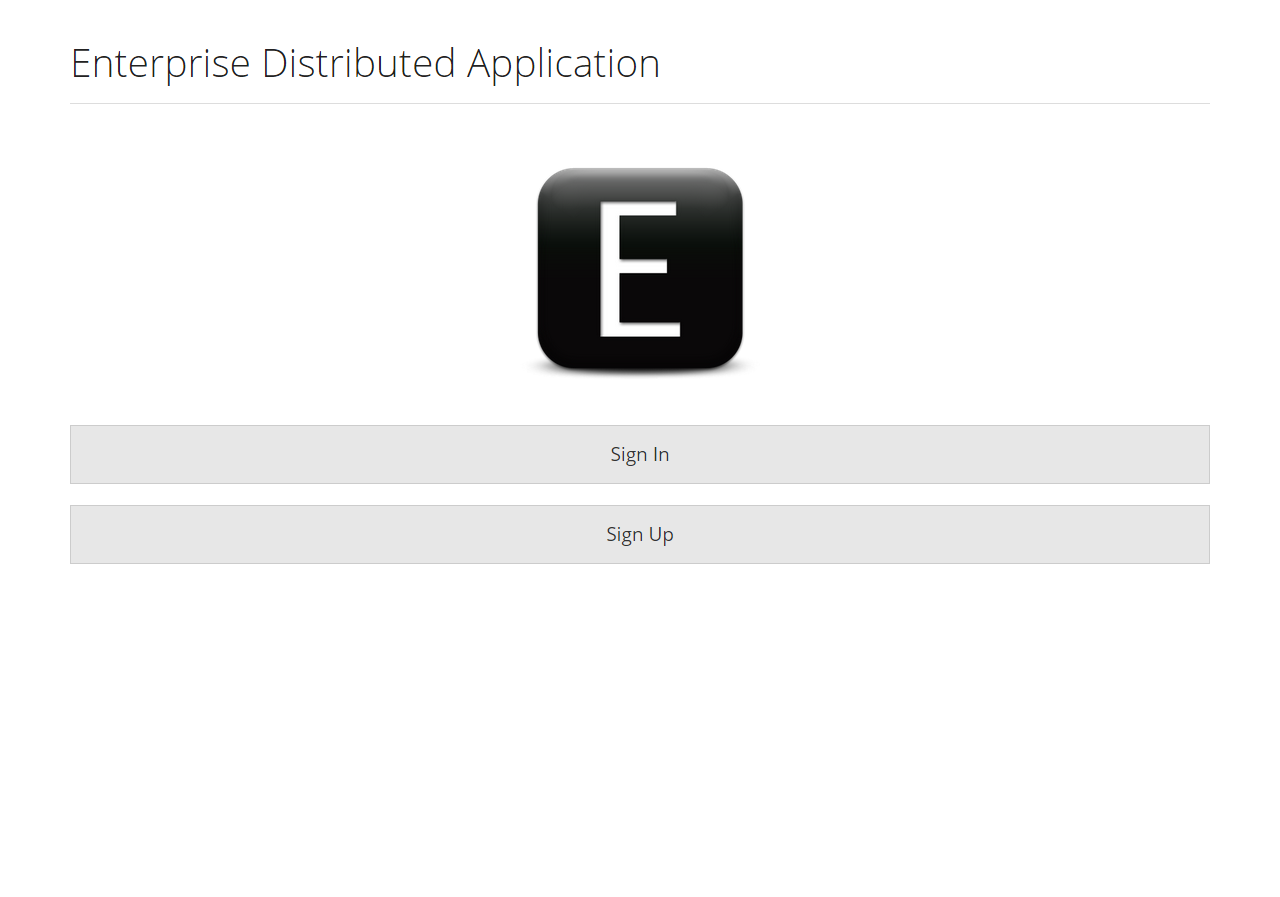
\includegraphics[width=0.8\textwidth]{Web_Initial.png}
    \caption{Interface gráfica da aplicação \textit{web} - Ecrã inicial.}
    \label{fig:c6}
\end{figure}

\begin{figure}[H]
    \centering
    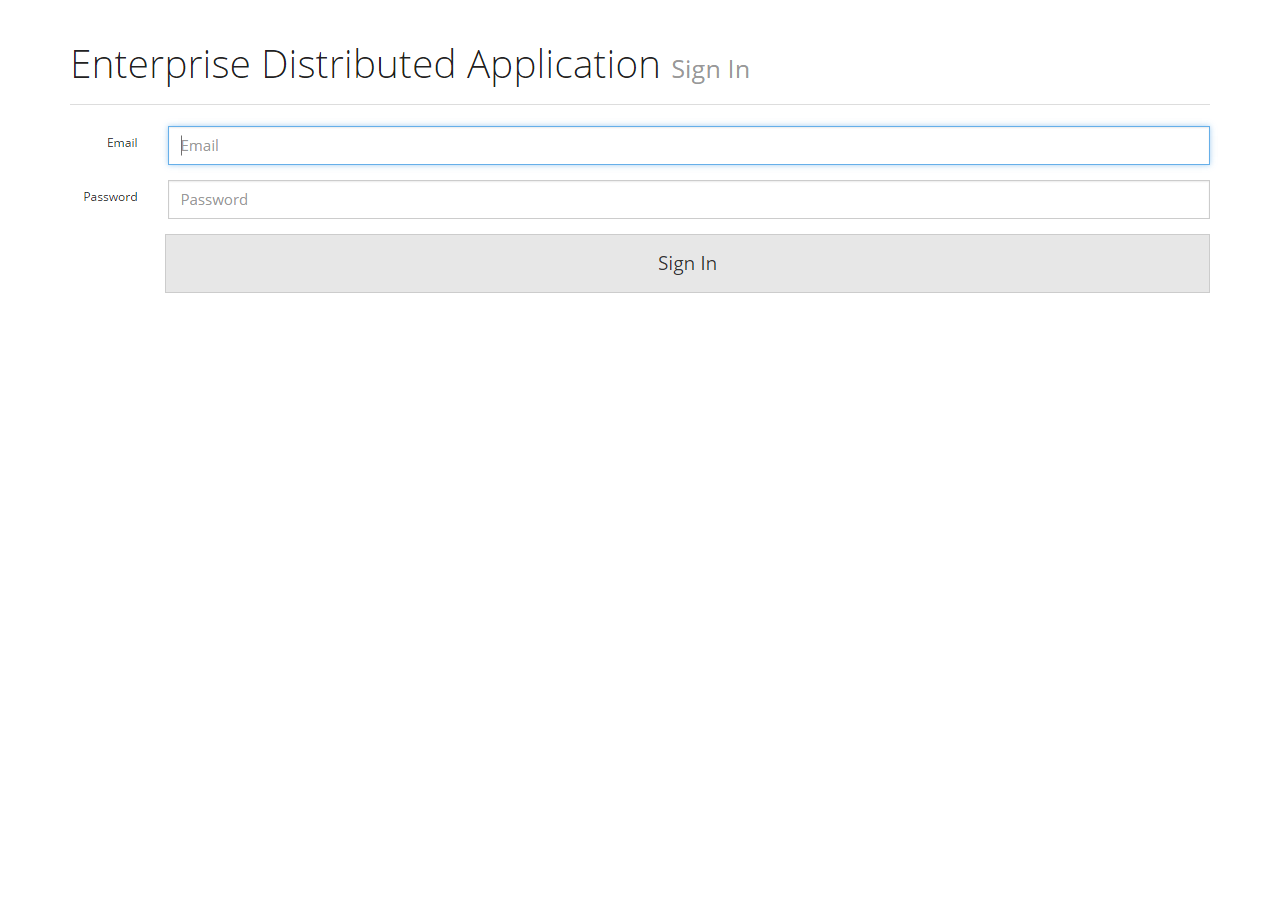
\includegraphics[width=0.8\textwidth]{Web_Login.png}
    \caption{Interface gráfica da aplicação \textit{web} - \textit{Login}.}
    \label{fig:c7}
\end{figure}

\begin{figure}[H]
    \centering
    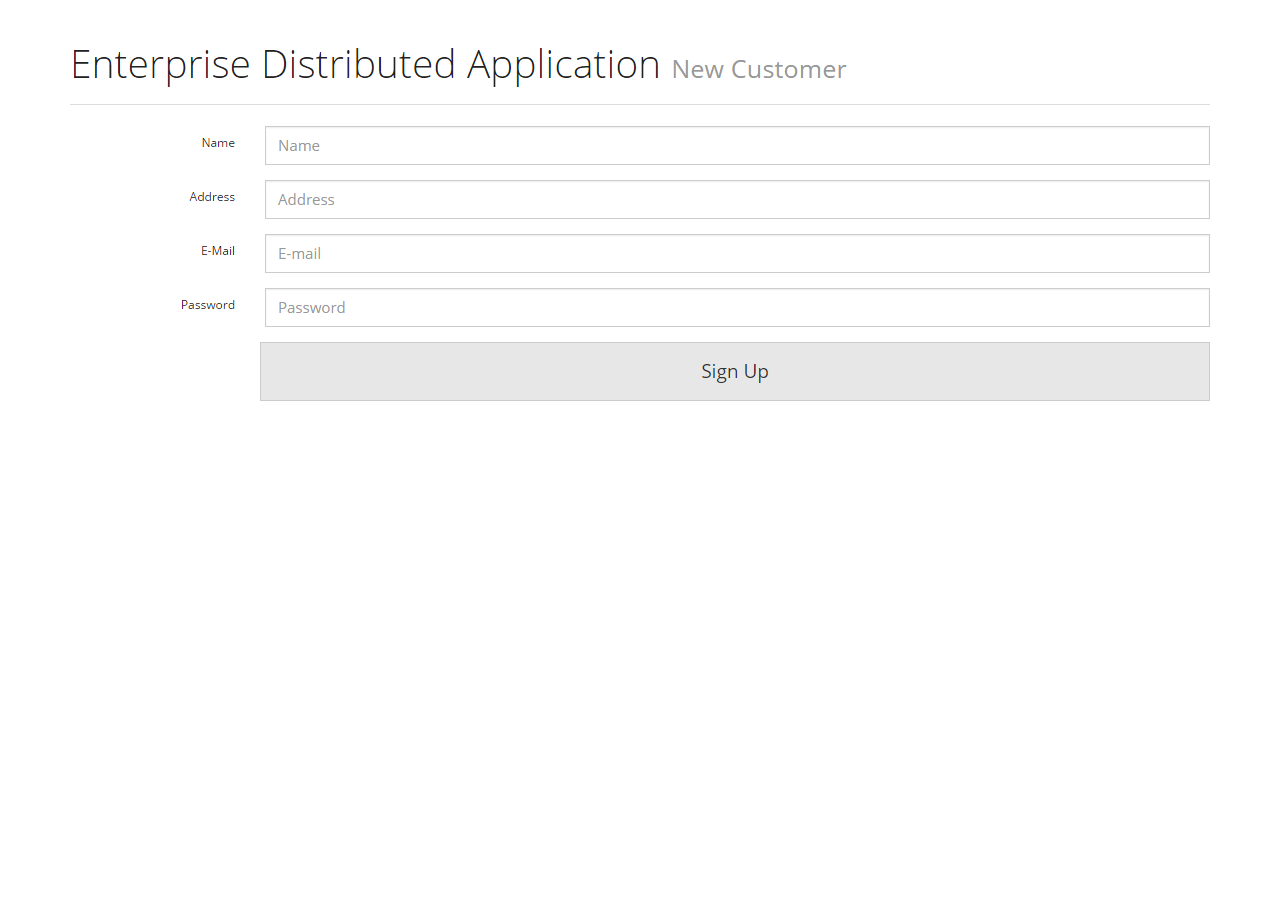
\includegraphics[width=0.8\textwidth]{Web_Register.png}
    \caption{Interface gráfica da aplicação \textit{web} - Registo.}
    \label{fig:c8}
\end{figure}

\begin{figure}[H]
    \centering
    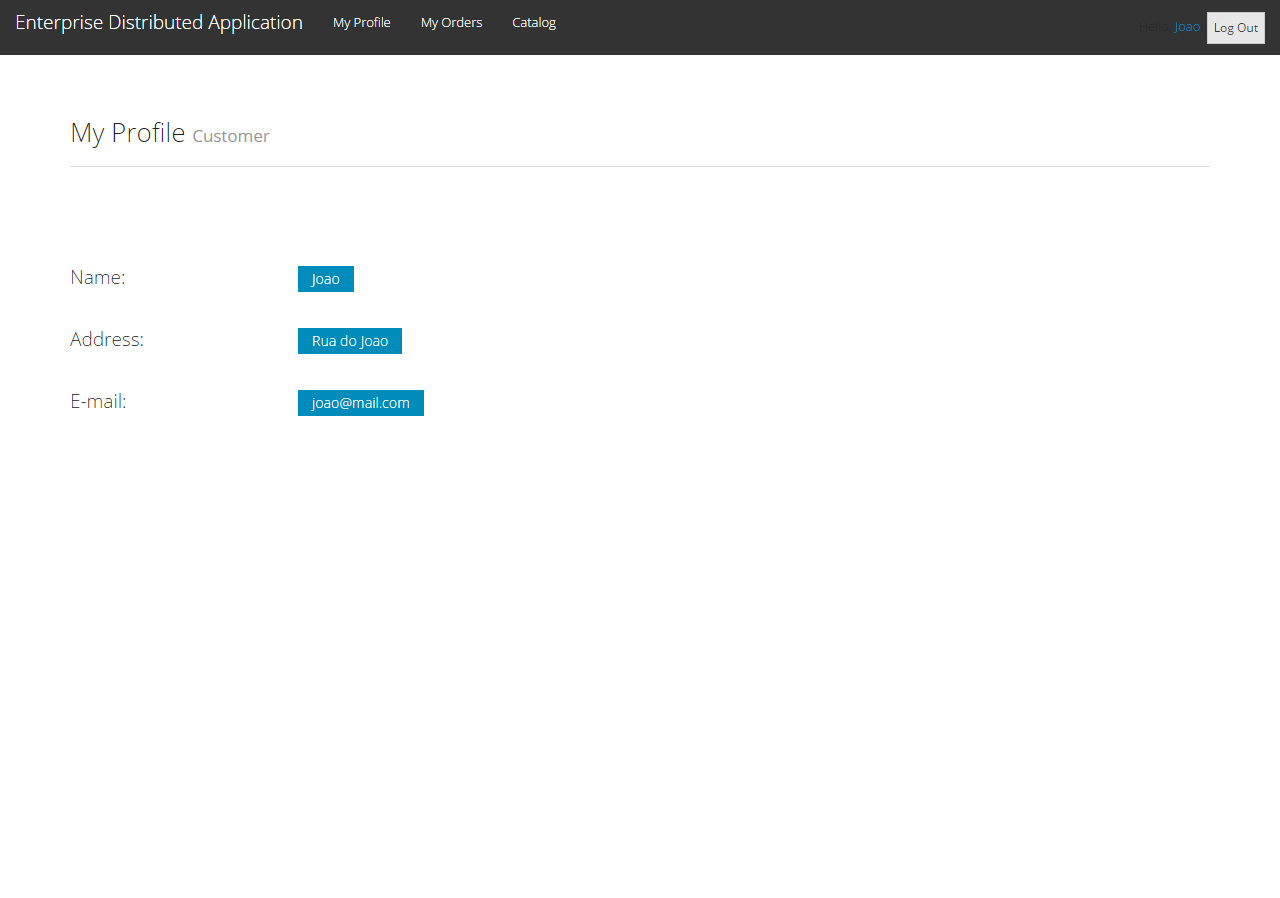
\includegraphics[width=0.8\textwidth]{Web_Profile.png}
    \caption{Interface gráfica da aplicação \textit{web} - Perfil.}
    \label{fig:c9}
\end{figure}

\begin{figure}[H]
    \centering
    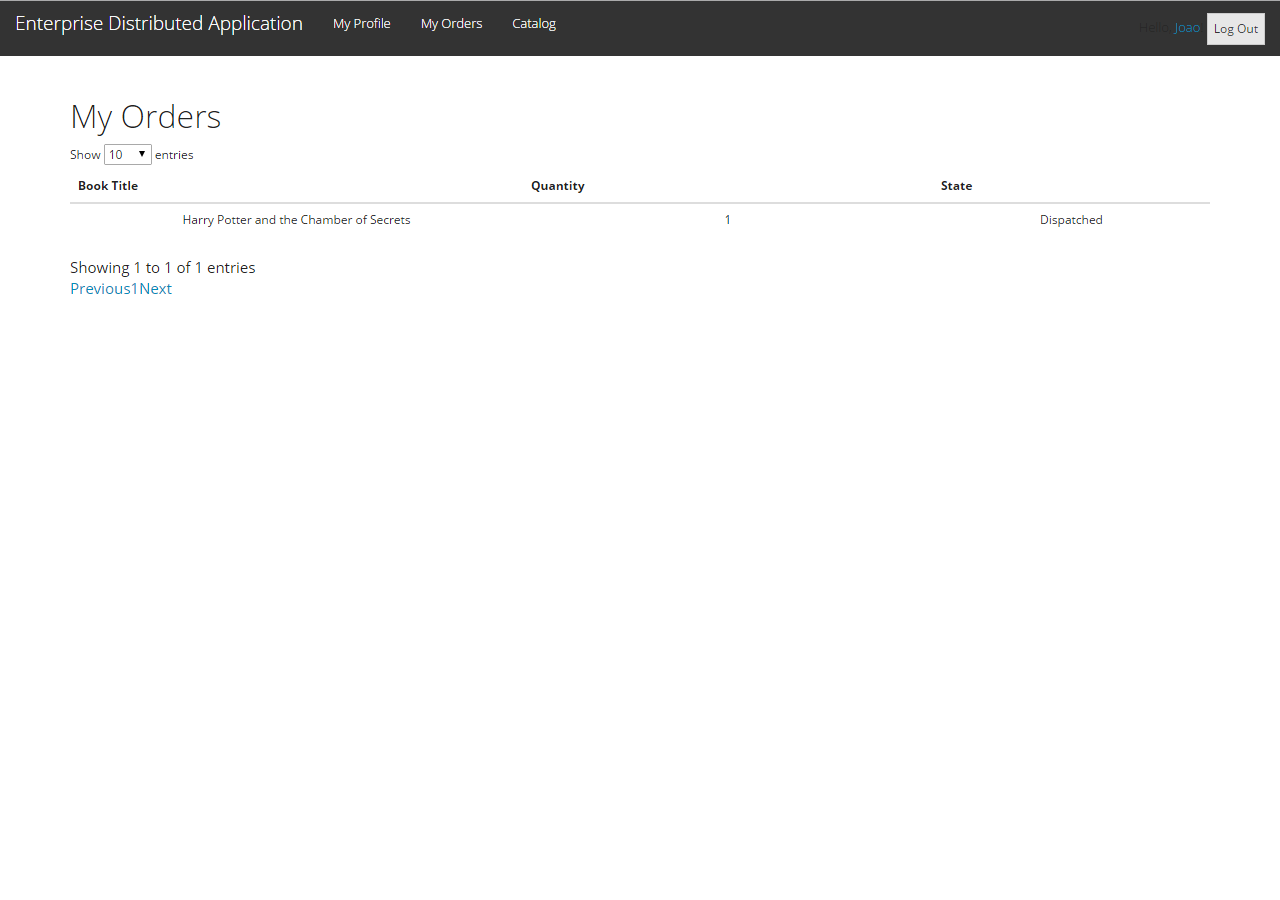
\includegraphics[width=0.8\textwidth]{Web_Orders.png}
    \caption{Interface gráfica da aplicação \textit{web} - Encomendas efetuadas.}
    \label{fig:c9}
\end{figure}

\begin{figure}[H]
    \centering
    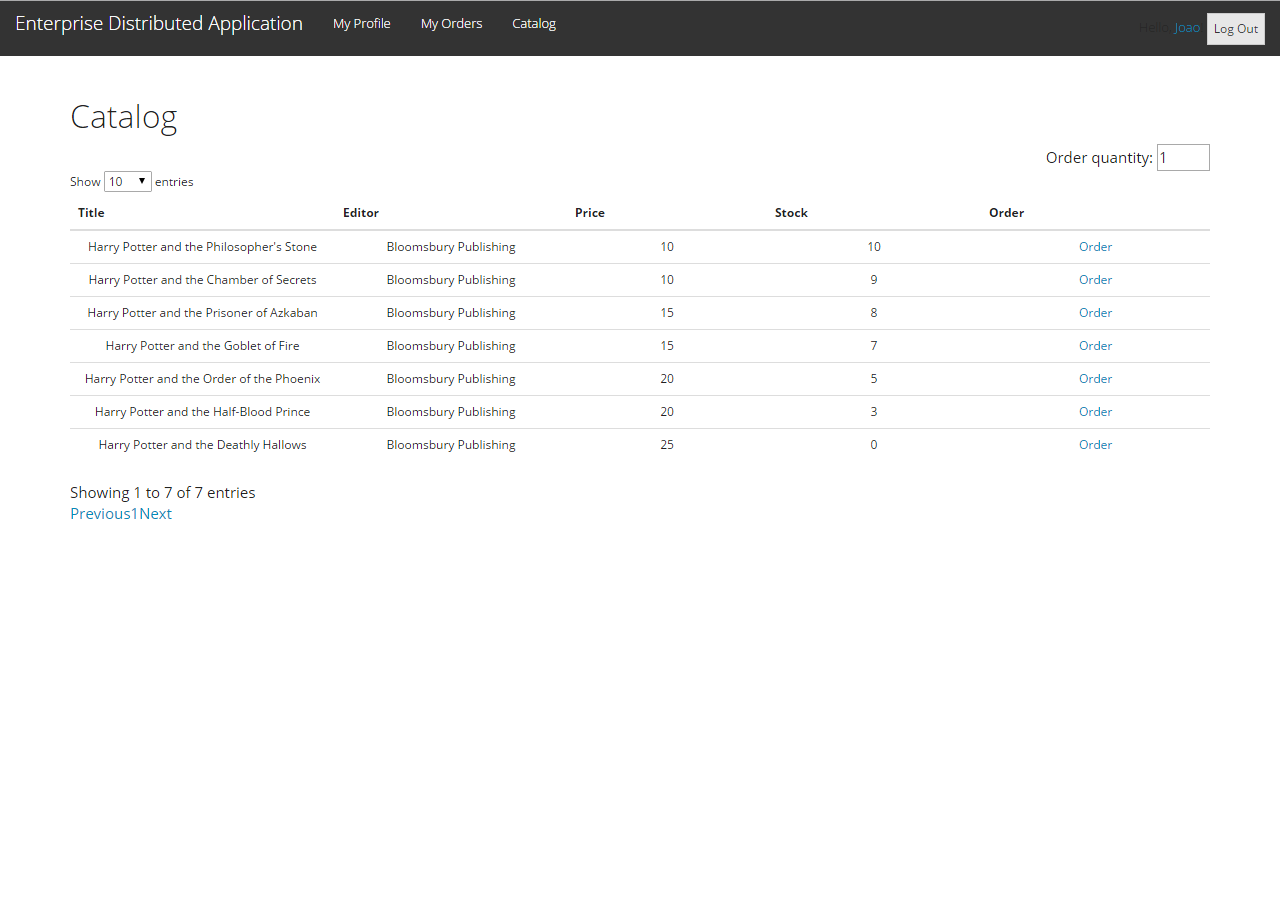
\includegraphics[width=0.8\textwidth]{Web_Catalog.png}
    \caption{Interface gráfica da aplicação \textit{web} - Consulta dos livros disponíveis em catálogo e possibilidade de fazer encomenda.}
    \label{fig:c10}
\end{figure}

Ao nível da interface gráfica desenvolvida para a aplicação \textit{web} numa primeira fase um ecrã onde é possível escolher entre fazer \textit{login} ou registar caso o utilizador ainda não seja cliente da loja, fig. \ref{fig:c6}.

Após o cliente fazer \textit{login} no sistema são disponibilizadas as opções de ver o seu perfil onde são apresentados os seus dados pessoais (fig \ref{fig:c8}), consultar as encomendas efetuadas (fig \ref{fig:c9}) e consultar o catálogo dos livros disponíveis para venda com a possibilidade fazer uma encomenda (fig \ref{fig:c10}).

\subsection{Casos de Uso}
\begin{figure}[H]
    \centering
    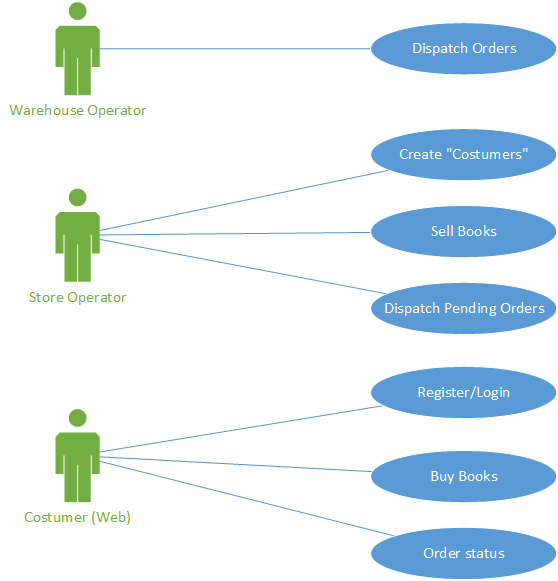
\includegraphics[width=0.8\textwidth]{use.png}
    \caption{Diagrama de casos de uso.}
    \label{fig:use}
\end{figure}


\section{Conclusão}

O sistema encontra-se desenvolvido com todas as funcionalidades solicitadas no enunciado do projeto, possibilitando ao utilizador uma utilização total do sistema.

\subsection*{Testes}

Para testar o correto funcionamento do sistema foram efetuadas várias experiências com diferentes clientes ligados a aplicação servidor, assim como, foram testados vários casos de falha ou do cliente e/ou servidor e garantida a persistência dos dados.

\subsection*{\textit{Deploy}}

O sistema pode ser utilizado colocando os servidores da loja e do armazém a correr e abrindo a aplicação cliente da loja e/ou a aplicação cliente \textit{web} disponível através do endereço /WebApp/index.php. Pode ser também aberto o projeto de \textit{Visual Studio} (\textit{EnterpriseDistributedApplication.sln}) e fazer \textit{Start} ao mesmo na interface do \textit{IDE}, no entanto, este não inclui a aplicação \textit{web}.

\section{Recursos}

\subsection{Bibliografia}
\begin{description}
\item Windows Communication Foundation .NET Framework 4.6 and 4.5, \url{https://msdn.microsoft.com/en-us/library/dd456779\%28v=vs.110\%29.aspx}.
\item Message Queuing (MSMQ), \url{https://msdn.microsoft.com/en-us/library/ms711472\%28v=vs.85\%29.aspx}.
\item Distribution and Integration Technologies, Miguel Monteiro, Faculdade de Engenharia da Universidade do Porto, \url{paginas.fe.up.pt/~apm/TDIN/}.
\end{description}
\subsection{\it{Software}}
\begin{description}
\item Visual Studio 2013 Ultimate, Microsoft, \url{http://www.visualstudio.com/}.
\item MongoDB, \url{https://www.mongodb.org/}.
\item SQLiteClient, Community, \url{http://www.nuget.org/packages/Community.CsharpSqlite.SQLiteClient/}.
\item NuGet, \url{http://www.nuget.org/}.
\item GitHub, \url{http://github.com/}.
\item MongoLab, \url{https://mongolab.com/}.
\end{description}


\end{document}
